\documentclass[12pt, twoside]{article}
\usepackage[letterpaper, margin=0.25in, head=30pt, headsep=0.1in]{geometry}
\usepackage[english]{babel}
\usepackage[utf8]{inputenc}
\usepackage{amsmath}
\usepackage{amsfonts}
\usepackage{amssymb}
\usepackage{tikz}
\usetikzlibrary{quotes, angles}

\usepackage{graphicx}
\usepackage{enumitem}
\usepackage{multicol}

%\usepackage{pgfplots}
%\pgfplotsset{width=10cm,compat=1.9}
%\usepgfplotslibrary{statistics}
%\usepackage{pgfplotstable}
%\usepackage{tkz-fct}
%\usepackage{venndiagram}

\usepackage{fancyhdr}
\pagestyle{fancy}
\fancyhf{}
\renewcommand{\headrulewidth}{0pt} % disable the underline of the header
\raggedbottom
\newif\ifmeta
\metatrue %print standards and topics tags

\title{Math AI Worksheet Generator and Formative Assessment System}
\author{Chris Huson}
\date{October 2020}

%\fancyhead[RE]{\thepage}
%\fancyhead[RO]{\thepage \\ Name: \hspace{3cm}}
%\fancyhead[L]{BECA / Dr. Huson / 10th Grade Geometry\\* 7 June 2019}
%
%\begin{document}
%\subsubsection*{13.7 Homework: Cross sections, distance applications}
%\fancyhead[L]{BECA / Dr. Huson / Geometry 03-Volume+angle-bisectors\\* pset ID: 34}

\begin{document}

\subsubsection*{3.5 ReQuiz review, angle addition}
\begin{enumerate}

  \item Type your answers. Use the less than key (``$<$'') to represent an angle, followed by three letters. \vspace{0.25cm}
  \begin{enumerate}
    \item Name a right angle: \rule{4cm}{0.15mm} \bigskip
    \item Name the angle vertical to $\angle LXM$: \rule{4cm}{0.15mm}  \bigskip 
    \item Name the ray opposite to $\overrightarrow{XJ}$: \rule{4cm}{0.15mm} \bigskip
    \item What is the measure of $\angle KXM$?  \rule{4cm}{0.15mm} \bigskip
    \item Spicy: Are $\angle JXL$ and $\angle LXM$ complementary, supplementary, or neither?
  \end{enumerate}
  \begin{center}
  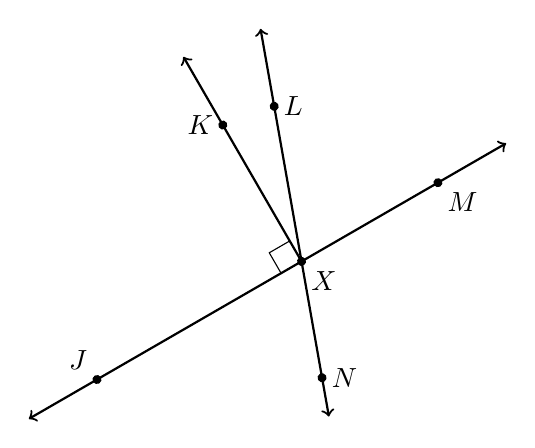
\begin{tikzpicture}[scale=1, rotate=30]
    \draw [<->, thick] (-110:2)--(0,0)--(70:3);
    \draw [<->, thick] (-4,0)--(3,0);
    \draw [->, thick] (0,0)--(0,3);
    \draw (0,0)++(-0.3,0)--++(0,0.3)--+(0.3,0);
    %\draw [fill] (-1,2.5) circle [radius=0.05] node[left ]{$B$};
    \draw [fill] (70:2) circle [radius=0.05] node[right]{$L$};
    \draw [fill] (-3,0) circle [radius=0.05] node[above left]{$J$}; 
    \draw [fill] (0,0) circle [radius=0.05] node[below right]{$X$};
    \draw [fill] (0,2) circle [radius=0.05] node[left]{$K$};
    \draw [fill] (2,0) circle [radius=0.05] node[below right]{$M$};
    \draw [fill] (-110:1.5) circle [radius=0.05] node[right]{$N$};
  \end{tikzpicture}
  \end{center}

\newpage
\item Demonstrate your ability to classify angles and use standard terminology.
\begin{enumerate}
  \item The given angle $\angle UVW$ is which of the following: acute, obtuse, or right?
  \begin{center}
    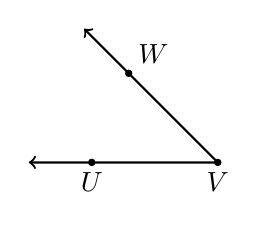
\begin{tikzpicture}[scale=.8]
      \draw  [<->, thick] (-3,0)--(0,0)--(135:3);
      \draw [fill] (-2,0) circle [radius=0.05] node[below]{$U$};
      \draw [fill] (0,0) circle [radius=0.05] node[below]{$V$};
      \draw [fill] (135:2) circle [radius=0.05] node[above right]{$W$};
    \end{tikzpicture}
  \end{center}
  \item Which of the following are true with respect to the angle, $m\angle PQR$?
  \begin{multicols}{2}
    True \hspace{0.25cm} False \hspace{0.25cm} It is an acute angle \\[0.5cm]
    True \hspace{0.25cm} False \hspace{0.25cm} It's measure is $90^\circ$\\[0.5cm]
    True \hspace{0.25cm} False \hspace{0.25cm} $\overrightarrow{PQ} \perp \overrightarrow{QR}$ \\[0.5cm]
    \columnbreak
    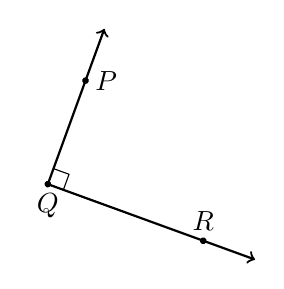
\begin{tikzpicture}[scale=0.7, rotate=-20]
      \draw [<->, thick] (4,0)--(0,0)--(0,3);
      \draw (0,0)++(0.3,0)--++(0,0.3)--+(-0.3,0);
      %\draw [fill] (-1,2.5) circle [radius=0.05] node[left ]{$B$};
      \draw [fill] (0,0) circle [radius=0.05] node[below]{$Q$};
      \draw [fill] (0,2) circle [radius=0.05] node[right]{$P$};
      \draw [fill] (3,0) circle [radius=0.05] node[above]{$R$};
    \end{tikzpicture}
  \end{multicols}
  \item What is sum of the degree measures of this linear pair, $\angle ABD$ and $\angle CBD$?
  \begin{center}
    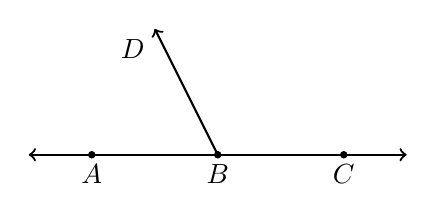
\begin{tikzpicture}[scale=.8, rotate=0]
      \draw  [<->, thick] (-3,0)--(3,0);
      \draw [->, thick] (0,0)--(-1, 2) node[below left]{$D$};
      \draw [fill] (-2,0) circle [radius=0.05] node[below]{$A$};
      \draw [fill] (0,0) circle [radius=0.05] node[below]{$B$};
      \draw [fill] (2,0) circle [radius=0.05] node[below]{$C$};
    \end{tikzpicture}
  \end{center}

  \end{enumerate}

\newpage
  \item As shown below, two lines intersect making four angles: $\angle 1$, $\angle 2$, $\angle 3$, and $\angle 4$.
  
    \begin{multicols}{2}
      Given $m\angle 2 = 110^\circ$.  
      \begin{enumerate}
        \item Find $m\angle 1$ \vspace{2cm}
        \item Find $m\angle 4$ \vspace{2cm}
      \end{enumerate}
      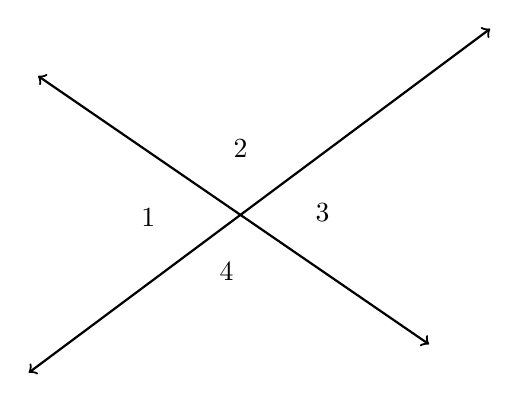
\begin{tikzpicture}[scale=0.7, rotate=20]
      \draw [<->, thick] (0,-1.5)--(10,1.5);
      \draw [<->, thick] (2,3.5)--(7,-3.5);
      \node at (3,.4){1};
      \node at (6,-.6){3};
      \node at (5,1){2};
      \node at (4,-1){4};
    \end{tikzpicture}
    \end{multicols}

\newpage
\subsubsection*{Angle addition situations}

\item Apply the Angle Addition postulate. Write and equation to support your work.
  \begin{multicols}{2}
    Given $m\angle CBD = 25^\circ$, $m\angle ABC = 90^\circ$. \\[0.5cm]
    Find $m \angle ABD$. \\
    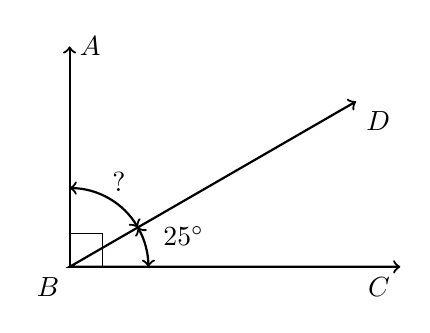
\begin{tikzpicture}[scale=1.4]
      \draw [<->, thick]
        (0:3) coordinate (a) node[below left] {$C$}
        -- (0,0) coordinate (b) node[below left] {$B$}
        -- (30:3) coordinate (c) node[below right] {$D$}
        pic["$25^\circ$", <->, draw=black, angle eccentricity=1.5, angle radius=1cm]
        {angle=a--b--c};
        \draw [<-, thick]
        (90:2) coordinate (d) node[right] {$A$}
        -- (0,0) coordinate (e)
        pic["$?$", <->, draw=black, angle eccentricity=1.25, angle radius=1cm]
        {angle=c--e--d};
      \draw (0,0)++(0.3,0)--++(0,0.3)--+(-0.3,0);
    \end{tikzpicture}
  \end{multicols}

\newpage
\item A linear pair is formed by two angles, $m\angle RUT = 2x+15$ and $m\angle SUT = 65^\circ$. \\[0.5cm] 
  Write an equation, then solve for $x$. \vspace{0.5cm}
    \begin{flushright}
      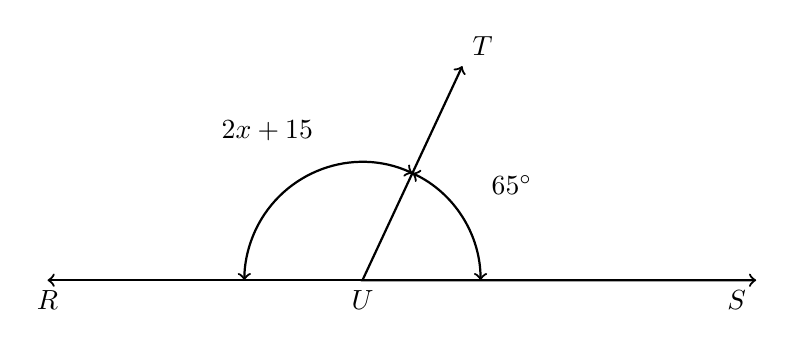
\begin{tikzpicture}[scale=1]
        \draw [<->, thick]
          (0:5) coordinate (a) node[below left] {$S$}
          -- (0,0) coordinate (b) node[below] {$U$}
          -- (65:3) coordinate (c) node[above right] {$T$}
          pic["$65^\circ$", <->, draw=black, angle eccentricity=1.5, angle radius=1.5cm]
          {angle=a--b--c};
          \draw [<-, thick]
          (180:4) coordinate (d) node[below] {$R$}
          -- (0,0) coordinate (e)
          pic["$2x+15$", <->, draw=black, angle eccentricity=1.5, angle radius=1.5cm]
          {angle=c--e--d};
          %\draw [->, thick] (0,0)--(-180:2) node[below right]{$A$};
          %\draw (0,0)++(-0.3,0)--++(0,0.3)--+(0.3,0);
      \end{tikzpicture}
    \end{flushright}
     
  \newpage
  \item Given $m\angle ABD = x+20$, $m\angle DBC = 4x$, and $m \angle ABC = 120^\circ$, as shown. \\[0.25cm]
  Write an equation and solve for $x$.
\begin{flushright}
      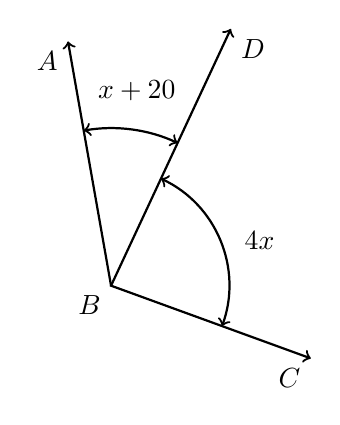
\begin{tikzpicture}[scale=1.8]
        \draw [<->, thick]
          (-20:1.5) coordinate (a) node[below left] {$C$}
          -- (0,0) coordinate (b) node[below left] {$B$}
          -- (65:2) coordinate (c) node[below right] {$D$}
          pic["\hspace{1cm}$4x$", <->, draw=black, angle eccentricity=1, angle radius=1.5cm]
          {angle=a--b--c};
          \draw [<-, thick]
          (100:1.75) coordinate (d) node[below left] {$A$}
          -- (0,0) coordinate (e)
          pic["$x+20$", <->, draw=black, angle eccentricity=1.25, angle radius=2cm]
          {angle=c--e--d};
      \end{tikzpicture}
    \end{flushright}
    Show your check for full credit.

  \newpage
  \item Given $\overrightarrow{BD} \perp \overleftrightarrow{ABC}$, $m\angle DBE = 2x$, and $m\angle EBC = x - 15^\circ$, as shown below. \\[0.5cm] 
  Write an equation and solve for $x$.
    \begin{flushright}
      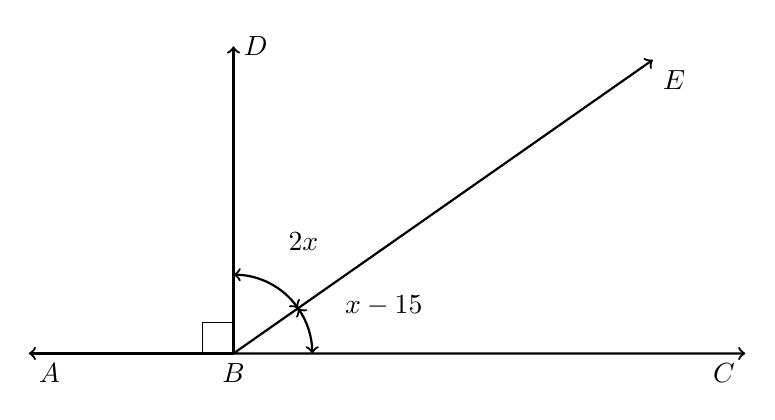
\begin{tikzpicture}[scale=1.3]
        \draw [<->, thick]
          (0:5) coordinate (a) node[below left] {$C$}
          -- (0,0) coordinate (b) node[below] {$B$}
          -- (35:5) coordinate (c) node[below right] {$E$}
          pic["$x-15$", <->, draw=black, angle eccentricity=2, angle radius=1cm]
          {angle=a--b--c};
          \draw [<-, thick]
          (90:3) coordinate (d) node[right] {$D$}
          -- (0,0) coordinate (e)
          pic["\hspace{0.3cm}$2x$", <->, draw=black, angle eccentricity=1.6, angle radius=1cm]
          {angle=c--e--d};
          \draw [->, thick] (0,0)--(-180:2) node[below right]{$A$};
          \draw (0,0)++(-0.3,0)--++(0,0.3)--+(0.3,0);
      \end{tikzpicture}
    \end{flushright}
 
  \newpage
  \item In the diagram shown, $\overrightarrow{BD} \perp \overleftrightarrow{ABC}$ and angle measures are given. \\[0.5cm] 
  Find $x$. Show the check for full credit.\vspace{0.5cm}
    \begin{multicols}{2}
      $m\angle DBE = 4x+4^\circ$ \\[0.25cm]
      $m\angle EBC = 9x-5^\circ$ \\[0.25cm]
      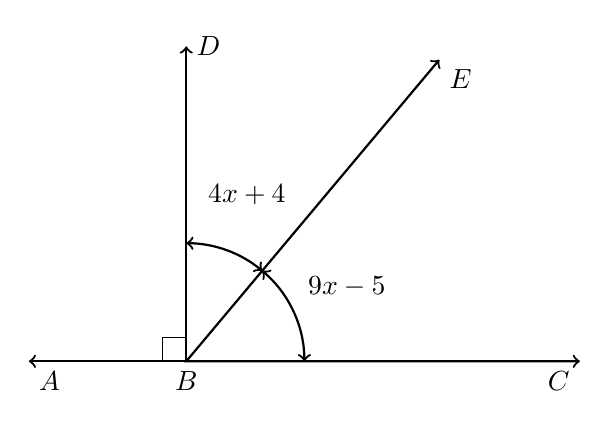
\begin{tikzpicture}[scale=1]
        \draw [<->, thick]
          (0:5) coordinate (a) node[below left] {$C$}
          -- (0,0) coordinate (b) node[below] {$B$}
          -- (50:5) coordinate (c) node[below right] {$E$}
          pic["$9x-5$", <->, draw=black, angle eccentricity=1.5, angle radius=1.5cm]
          {angle=a--b--c};
          \draw [<-, thick]
          (90:4) coordinate (d) node[right] {$D$}
          -- (0,0) coordinate (e)
          pic["$4x+4$", <->, draw=black, angle eccentricity=1.5, angle radius=1.5cm]
          {angle=c--e--d};
          \draw [->, thick] (0,0)--(-180:2) node[below right]{$A$};
          \draw (0,0)++(-0.3,0)--++(0,0.3)--+(0.3,0);
      \end{tikzpicture}
    \end{multicols}

  \newpage
  \item Spicy: Given $\overleftrightarrow{ABC}$, right angle $\angle DBE$, $m\angle ABE = 3x+6$, and $m\angle DBC = 2x-1$. \\[0.5cm] 
  Find $m\angle ABE$. \vspace{0.5cm}
    \begin{flushright}
      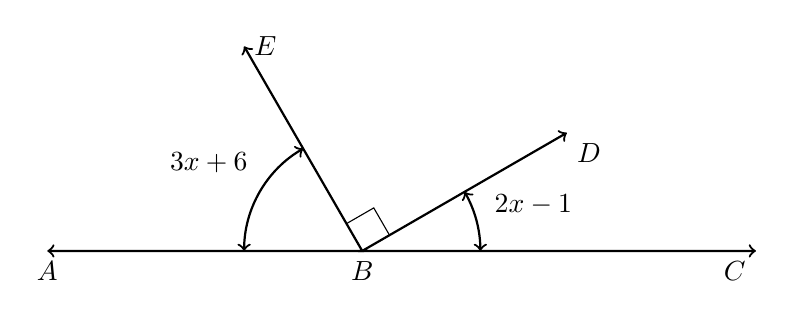
\begin{tikzpicture}[scale=1, rotate=30]
        \draw [<->, thick]
          (-30:5) coordinate (a) node[below left] {$C$}
          -- (0,0) coordinate (b) node[below] {$B$}
          -- (3,0) coordinate (c) node[below right] {$D$}
          pic["$2x-1$", <->, draw=black, angle eccentricity=1.5, angle radius=1.5cm]
          {angle=a--b--c};
          \draw [<->, thick]
          (150:4) coordinate (d) node[below] {$A$}
          -- (0,0) -- (0, 3) coordinate (e) node[right] {$E$}
          pic["$3x+6$", <->, draw=black, angle eccentricity=1.5, angle radius=1.5cm]
          {angle=e--b--d};
          \draw (0,0)++(0.4,0)--++(0,0.4)--+(-0.4,0);
      \end{tikzpicture}
    \end{flushright}

  \newpage
  \item Spicy: Ray $\overrightarrow{BF}$ is the angle bisector of $\angle ABC$. Given that the angle measures are $m\angle ABF = 7x-14$ and $m\angle CBF = 5x+10$. \\[0.5cm] 
  Find $x$. \vspace{0.5cm}
    \begin{flushright}
      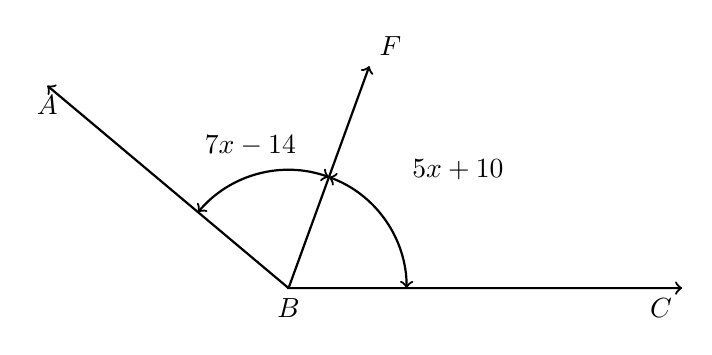
\begin{tikzpicture}[scale=1]
        \draw [<->, thick]
          (0:5) coordinate (a) node[below left] {$C$}
          -- (0,0) coordinate (b) node[below] {$B$}
          -- (70:3) coordinate (c) node[above right] {$F$}
          pic["$5x+10$", <->, draw=black, angle eccentricity=1.75, angle radius=1.5cm]
          {angle=a--b--c};
          \draw [<-, thick]
          (140:4) coordinate (d) node[below] {$A$}
          -- (0,0) coordinate (e)
          pic["$7x-14$", <->, draw=black, angle eccentricity=1.25, angle radius=1.5cm]
          {angle=c--e--d};
          %\draw [->, thick] (0,0)--(-180:2) node[below right]{$A$};
          %\draw (0,0)++(-0.3,0)--++(0,0.3)--+(0.3,0);
      \end{tikzpicture}
    \end{flushright}
      
  
\newpage
\item Spicy: Given $\overline{PQRS}$. $Q$ is the midpoint of $\overline{PS}$, and $R$ bisects $\overline{QS}$. \\[0.5cm] 
If $PR= 4 \frac{1}{2}$ find ${PS}$. Justify your answer.
  \begin{flushright}
      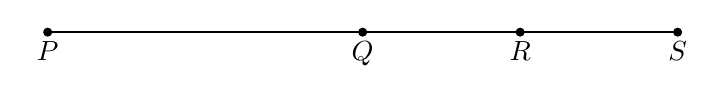
\begin{tikzpicture}
        \draw [-, thick] (0,0)--(8,0);
        \draw [fill] (0,0) circle [radius=0.05] node[below]{$P$};
        \draw [fill] (4,0) circle [radius=0.05] node[below]{$Q$};
        \draw [fill] (6,0) circle [radius=0.05] node[below]{$R$};
        \draw [fill] (8,0) circle [radius=0.05] node[below]{$S$};
      \end{tikzpicture}
    \end{flushright}

\newpage
\item Spicy: Given $A(0)$ and $T(2)$, as shown on the number line. $T$ is one of the points that trisects $\overline{AB}$.  \\[0.25cm]
  Find $B$. For full credit, find both solutions.
  \begin{center}
    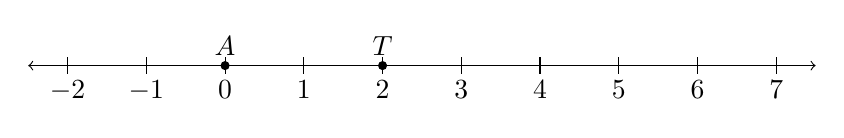
\begin{tikzpicture}
      \draw [<->] (-2.5,0)--(7.5,0);
      %\draw [-, thick] (0,0)--(2,0);
      \foreach \x in {-2,...,7} %2 leading for diff!=1
        \draw[shift={(\x,0)},color=black] (0pt,-3pt) -- (0pt,3pt) node[below=5pt]  {$\x$};
        \draw [fill] (0,0) circle [radius=0.05] node[above] {$A$};
        \draw [fill] (2,0) circle [radius=0.05] node[above] {$T$};
    \end{tikzpicture}
  \end{center}

\end{enumerate}
\end{document}